\section{Enabling Technologies}

A range of technologies developed over several years have enabled the evolution of NFV and Edge Computing. These technologies can be grouped among four planes of computing. This model is applicable to MEC as well as the related technology called NFV.

\begin{figure}[h!]
	\centering
    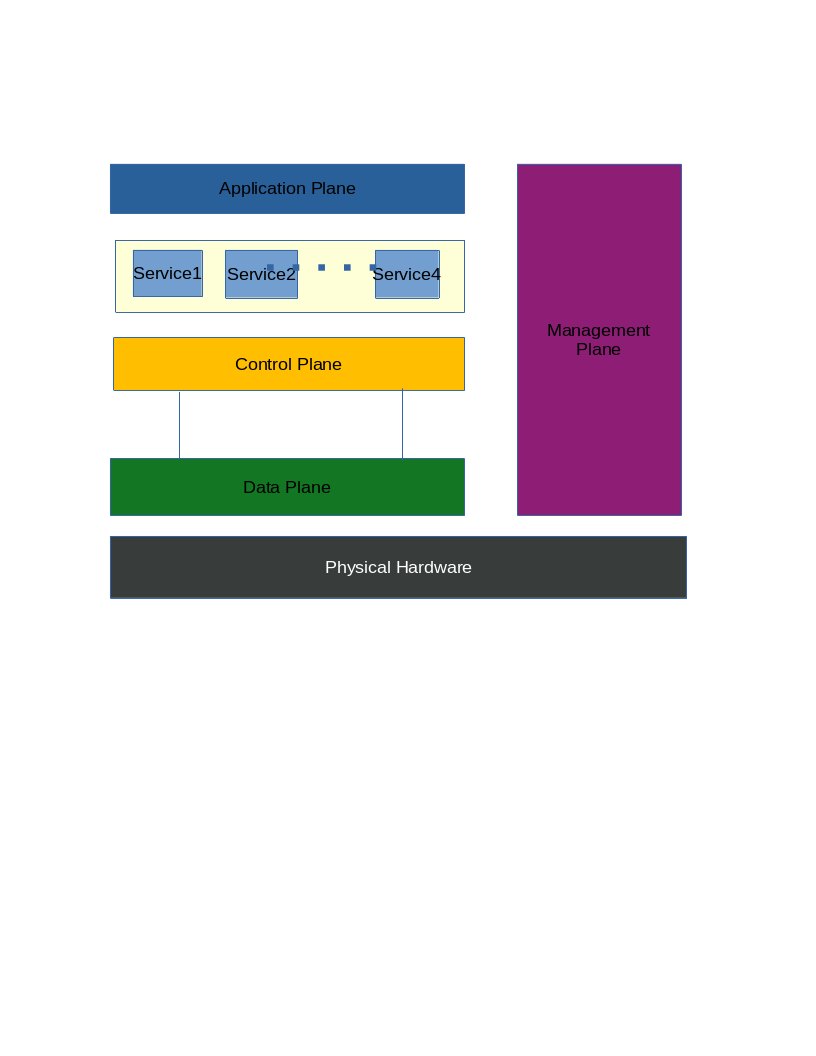
\includegraphics[width=0.7\textwidth]{planes_of_computing}
	\label{fig:7}
	\caption{Planes of NFV and MEC Architectures}
\end{figure}

These technologies can be grouped into 4 different planes based on their functionalities.

\begin{enumerate}
    \item Data Plane
	\begin{itemize}
	    \item Follows the forwarding logic and responsible for physically moving the packets in the network.
        \end{itemize}
    \item Control Plane
	\begin{itemize}
	    \item Computes the forwarding logic as required by the other planes and programs them to the Data plane and monitors the data plane.
        \end{itemize}
    \item Management Plane
	\begin{itemize}
	    \item Responsible for orchestration and management of resources as required by the services.
	\end{itemize}
    \item Application Plane
	\begin{itemize}
	    \item Makes use of the services through Service Abstraction and APIs from Management to deliver end-user applications.
	\end{itemize}
\end{enumerate}

NIST Cloud Computing group defines cloud computing \cite{nist} as "a model for enabling ubiquitous, convenient, on-demand network access to a shared pool of configurable computing resources that can be rapidly provisioned and released with minimal management effort or service provider interaction". It also enumerates three service models for cloud providers. 

\begin{enumerate}
    \item Infrastructure As A Service
        The provider provides infrastructure and APIs to the consumer to provision processing, storage and network resources allowing the consumer to run arbitrary applications and services.
    \item Platform as a Service
        The consumer can write applications using the programming languages, tools and libraries provided by the provider.
    \item Software As A Service
        The consumer runs the application provided by the provider using a suitable interface like a web-browser or a specialized program. 
\end{enumerate}

\begin{figure}[h!]
	\centering
    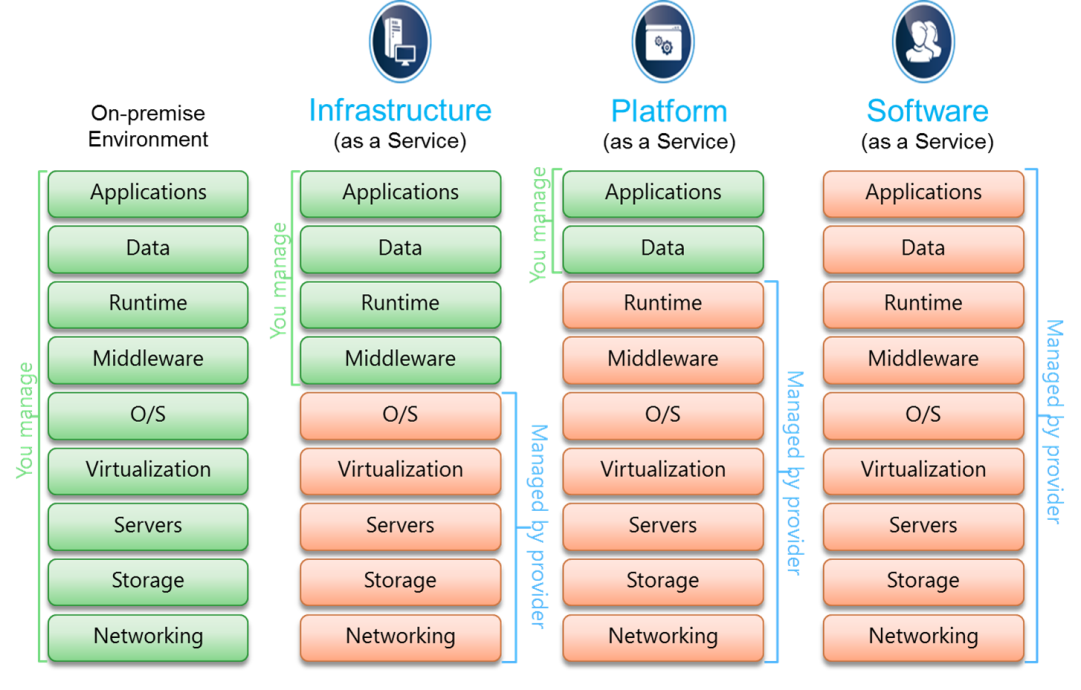
\includegraphics[width=0.9\textwidth]{cloud_service_model}
	\label{fig:8}
    \caption{Service Models for Cloud Computing \protect\cite{cloudservice}}
\end{figure}
